\subsection{Computation of derivatives}\label{sec:derivatives}
Computation of derivative quantities such as gradient and Laplacian is of fundamental importance in
data analysis. Since simulation data can rarely be captured by closed-form formulas, we use finite
differences. In this section, we use 32 bits (instead of 16) for quantization, to ensure enough
precision for finite differences. We always perform finite differences on the finest (original)
resolution. This decision avoids the problem of computing distances between quantities defined on
grids of different sizes, because we are unaware of any widely accepted solutions to this problem.
\autoref{sec:gradient} discusses gradient computation, and \autoref{sec:laplacian} discusses
computation of the Laplacian.

\subsubsection{Gradient}\label{sec:gradient}
For the gradient, we have experimented with three popular finite difference schemes using stencil
sizes of two, three, and five points in each dimension. We have foundno tangible differences in the
results, and therefore present results for the five-point stencil exlusively: $\frac{\partial
f}{\partial x}\approx \frac{1}{12}f(x-2)-\frac{2}{3}f(x-1)+\frac{2}{3}f(x+1)-\frac{1}{12}f(x+2)$. In
3D, the gradient at grid point $(x,y,z)$ is the vector $(\frac{\partial f}{\partial
x},\frac{\partial f}{\partial y}, \frac{\partial f}{\partial y})$. We use Algorithm~\ref{alg:greedy}
to compute a \emph{gradient-optimized} ($s_{grad-opt}$) stream that minimizes the difference between
the reconstructed gradient field and the original gradient field. The error at each grid point $x_i$
is the squared Euclidean length of the difference between two gradient vectors, that is,
$\norm{\nabla \tilde{f}(x_i)-\nabla f(x_i)}^2$, where $\tilde{f}$ is an approximation of $f$
at low bit rates. The overall error, defined over the whole field, is $e(\nabla \tilde{f},\nabla
f)=\sqrt{\frac{1}{n}\sum_{i=1}^{n}{\norm{\nabla \tilde{f}(x_i)-\nabla f(x_i)}^2}}$.

Using four data sets, we plot gradient error curves produced by $s_{lvl}$, $s_{bit}$, $s_{mag}$,
$s_{wav}$, $s_{grad-opt}$, and $s_{grad-sig}$ in \autoref{fig:gradient-error-comparison}. In
general, $s_{grad-opt} > s_{grad-sig} \approx s_{bit} > s_{wav} > s_{mag} > s_{lvl}$. This ordering
can also be seen in \autoref{fig:gradient-rendering-diff}, where the x-component of the gradient
field for \emph{tuburlence} is reconstructed and rendered, at 0.2 bps. Unlike in the RMSE case,
$s_{bit}$ produces better approximations of the gradient field, compared to $s_{wav}$. This
phenomenon is explained in \autoref{fig:bit-plane-vs-wavelet-norm-gradient}.

In \autoref{fig:bit-plane-vs-wavelet-norm-gradient}, a 1D line is extracted from \emph{plasma}, and
reconstructed using $s_{bit}$ and $s_{wav}$ at 0.6 bps. Because the coarse-scale coefficients in
$s_{bit}$ are not accurate enough, the reconstruction from $s_{bit}$ is inaccurate in areas of low
gradients. In constrast, the $s_{wav}$'s reconstruction is accurate in low-gradient areas, but lacks
the resolution to resolve the high-gradient areas. This is because $s_{wav}$ frequently intersperses
bits that improve resolution and bits that improve precision, unlike $s_{bit}$, which always stream
bits that improve resolution first. As such, $s_{wav}$ tends to produce a ``smoother''
reconstruction that, \emph{on average} (i.e., in terms of RMSE), is close to the original function.
$s_{bit}$, on the other hand, tends to capture well the function's shape (due to fine-scale bits),
but the whole function can be ``shifted'' slightly due to the lack of precision in coarse-scale
coefficients. However, the error caused by this shifting reduces significantly when taking gradient,
which cancels any constant shift. $s_{bit}$, therefore, works better than $s_{wav}$ for gradient
computation, thanks to its virtue of being able to better retain sharp features.

\duong{talk about the by-level, by-magnitude, and signature}.

\begin{figure}[h]
	\centering
	\subcaptionbox{boiler}{
	{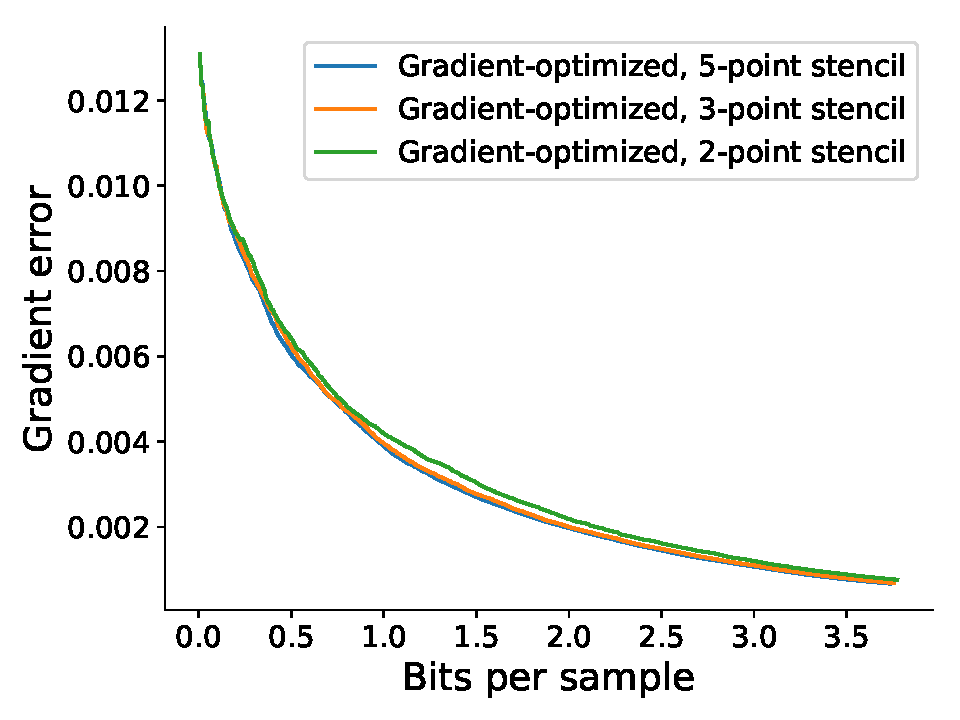
\includegraphics[width=0.48\linewidth]{gradient/gradient-optimized-boiler}}}
	\subcaptionbox{diffusivity}{
	{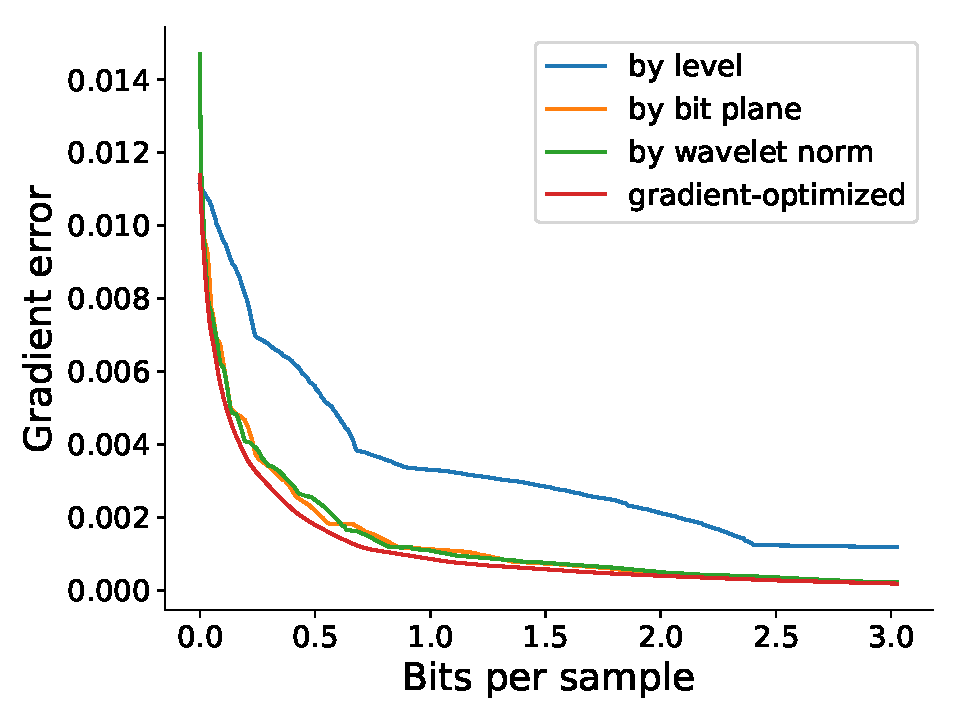
\includegraphics[width=0.48\linewidth]{gradient/gradient-optimized-diffusivity}}}
	\subcaptionbox{turbulence}{
	{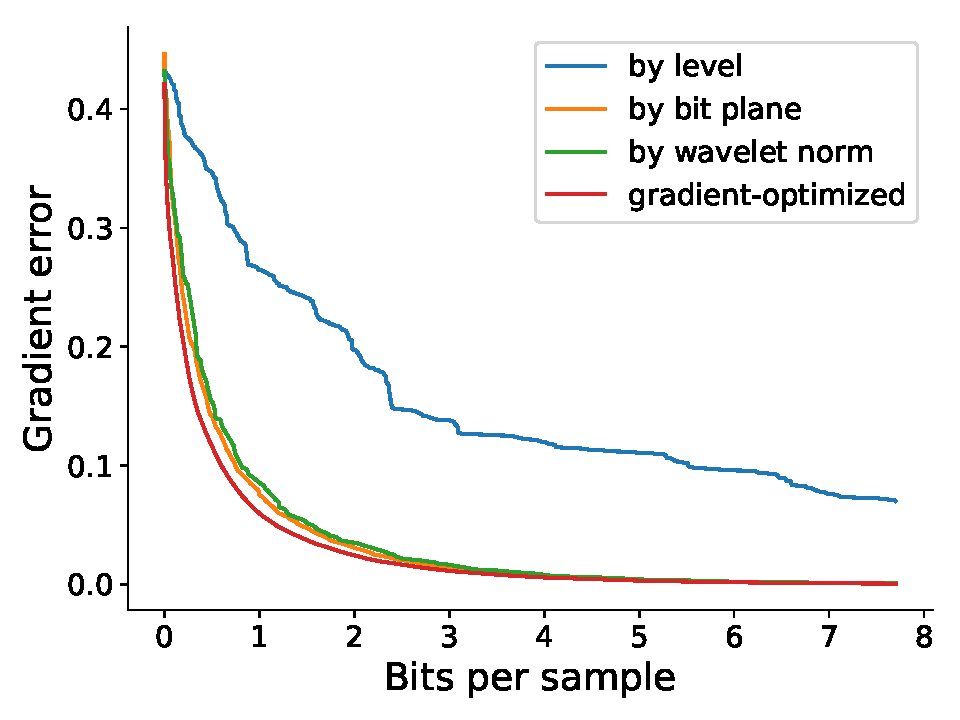
\includegraphics[width=0.48\linewidth]{gradient/gradient-optimized-turbulence}}}
	\subcaptionbox{pressure}{
	{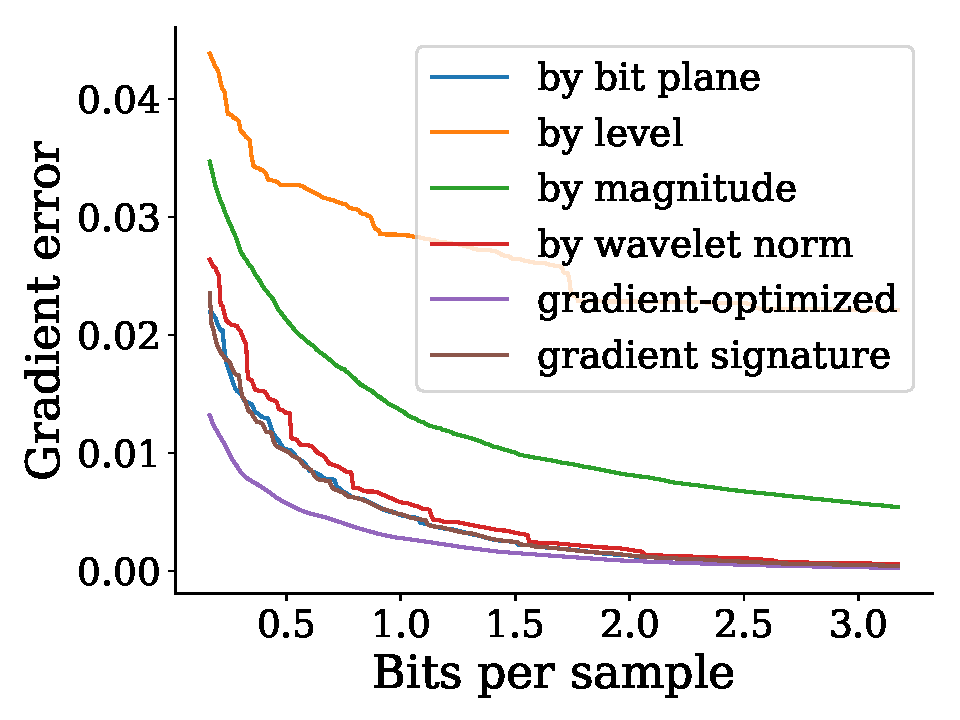
\includegraphics[width=0.48\linewidth]{gradient/gradient-optimized-pressure}}} \caption{Gradient
	error of reconstructed functions. Lower is better. Leading zero packets are removed, and the plots
	are truncated in the same way as in Figure \ref{fig:rmse-optimized}. The trend, in all cases, is
	$s_{grad-opt} > s_{grad-sig} \approx s_{bit} > s_{wav} > s_{mag} > s_{lvl}$.}
	\label{fig:gradient-error-comparison}
\end{figure}

\begin{figure}[h]
	\centering
	\subcaptionbox{\emph{by level} ($s_{lvl}$)}{
	{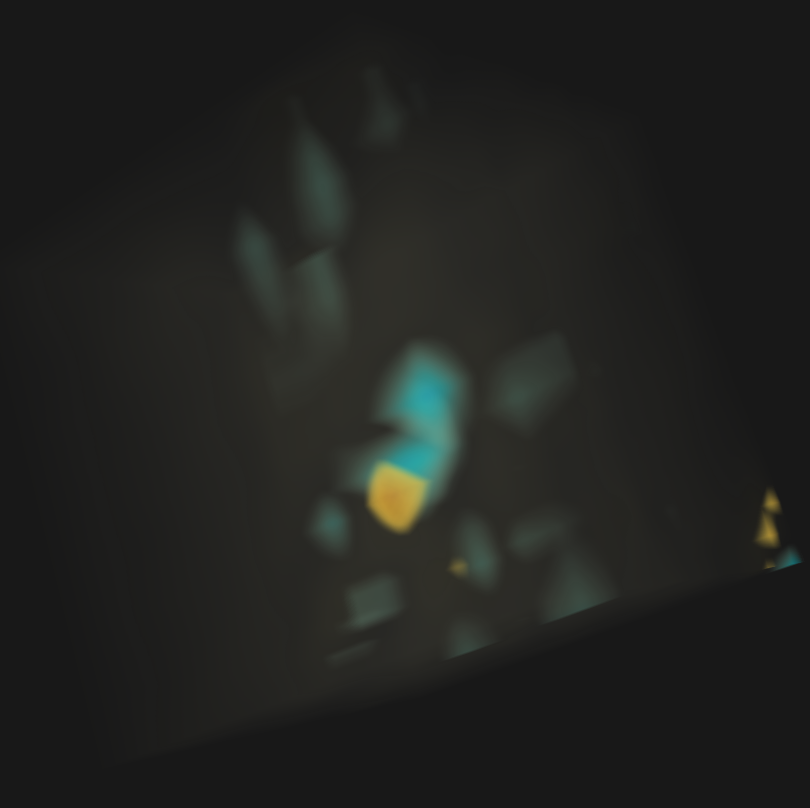
\includegraphics[width=0.31\linewidth]{gradient/gradient-turbulence-level}}}
	\subcaptionbox{\emph{by bit plane} ($s_{bit}$)}{
	{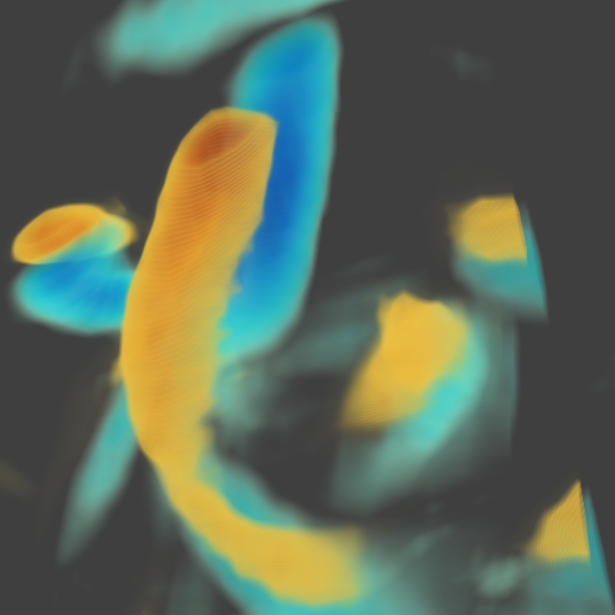
\includegraphics[width=0.31\linewidth]{gradient/gradient-turbulence-bit-plane}}}
	\subcaptionbox{\emph{by wavelet norm} ($s_{wav}$)}{
	{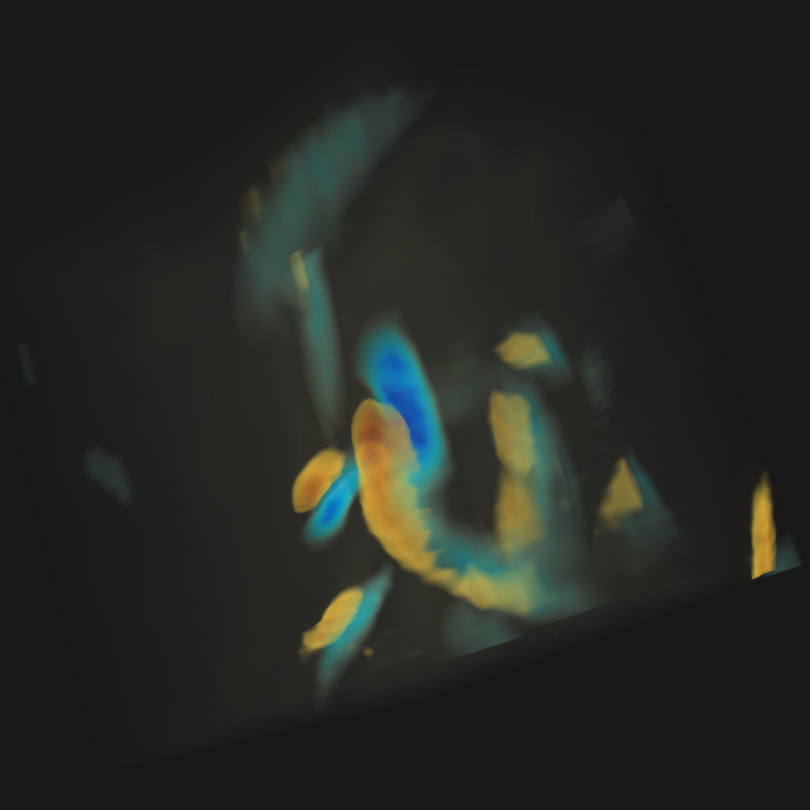
\includegraphics[width=0.31\linewidth]{gradient/gradient-turbulence-wavelet-norm}}}
	\subcaptionbox{\emph{by magnitude} ($s_{mag}$)}{
	{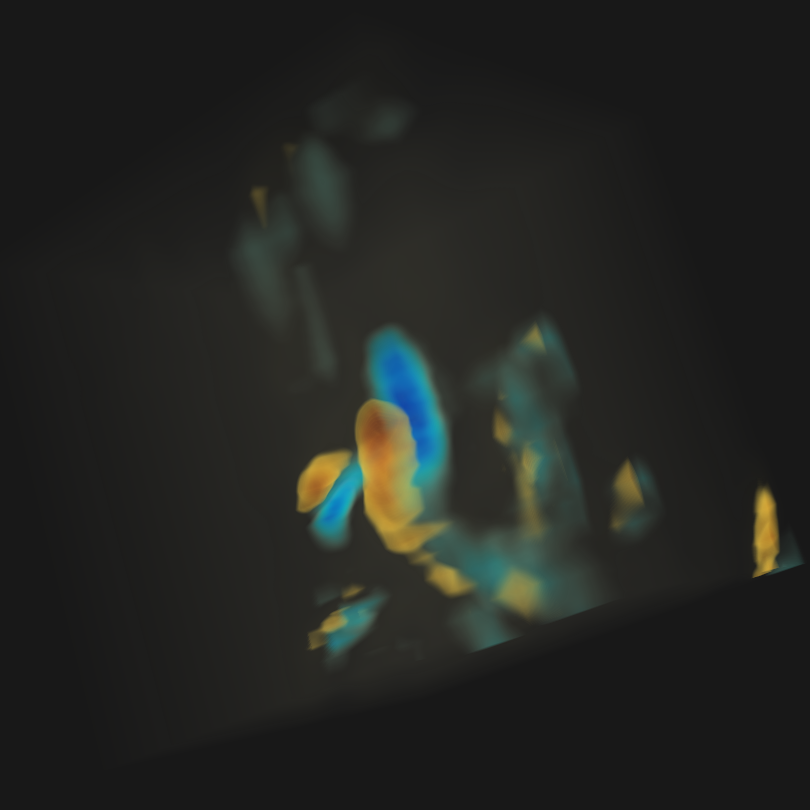
\includegraphics[width=0.31\linewidth]{gradient/gradient-turbulence-magnitude}}}
	\subcaptionbox{\emph{by signature} ($s_{grad-sig}$)}{
	{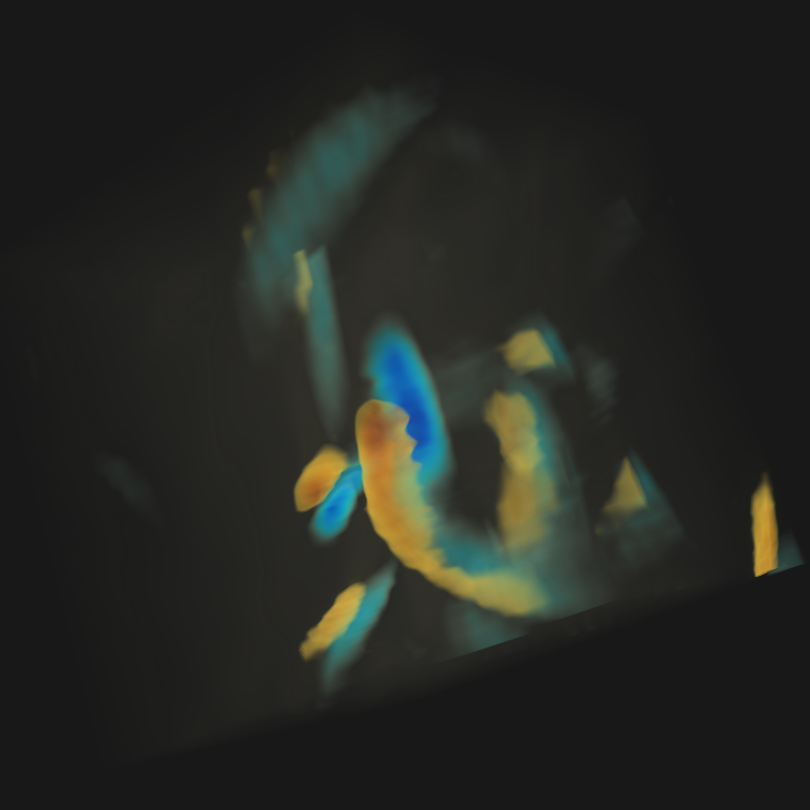
\includegraphics[width=0.31\linewidth]{gradient/gradient-turbulence-signature.png}}}
	\subcaptionbox{\emph{reference}}{
	{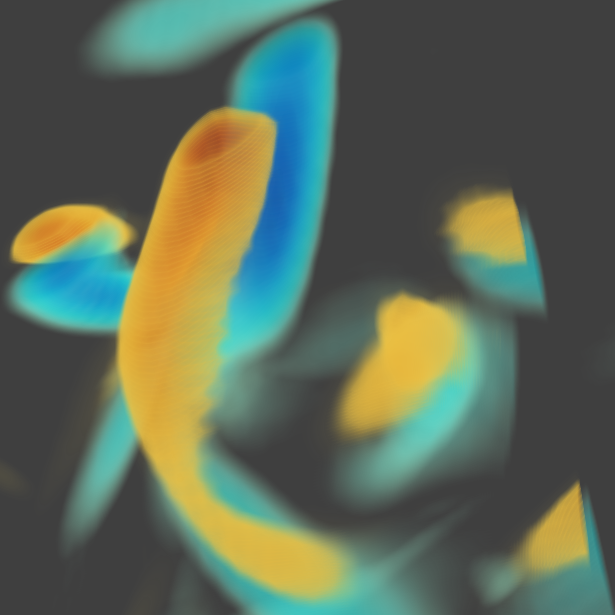
\includegraphics[width=0.31\linewidth]{gradient/gradient-turbulence-groundtruth.png}}}
	\caption{x-component of the ($64^3$) gradient field of \emph{turbulence}, reconstructed at 0.2
	bps. The gradient field produced by $s_{bit}$ is more accurate than one produced by either
	$s_{wav}$ or $s_{grad-sig}$ (compare orange features).}\label{fig:gradient-rendering-diff}
\end{figure}

\begin{figure}[h]
	\centering
	\subcaptionbox{$s_{bit}$}{
	{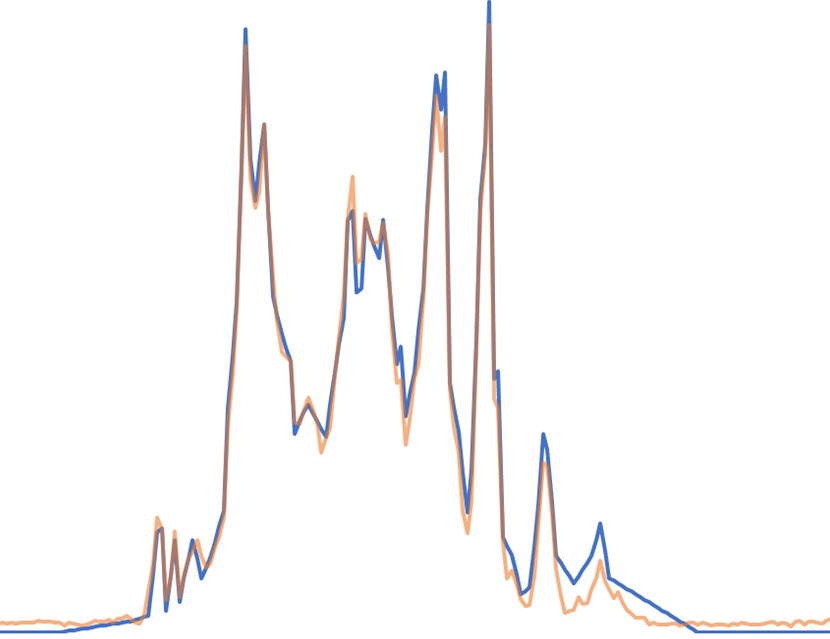
\includegraphics[width=0.48\linewidth]{gradient/gradient-bit-plane}}}
	\subcaptionbox{$s_{wav}$}{
	{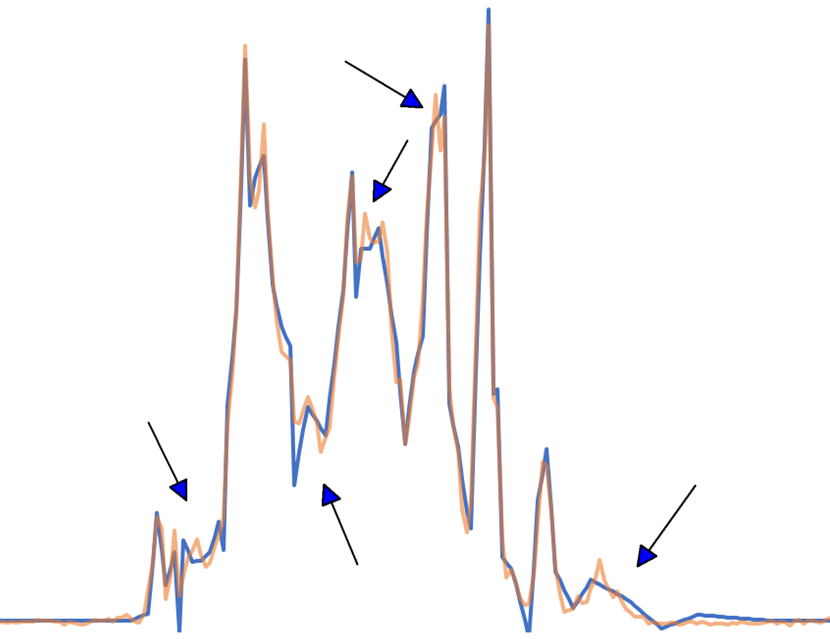
\includegraphics[width=0.48\linewidth]{gradient/gradient-wavelet-norm}}}
	\caption{A 1D line extracted from \emph{plasma}, and reconstructed using $s_{bit}$ and $s_{wav}$ at
	0.6 bps. The original data is in orange, whille the reconstructions are in blue. $s_{wav}$ captures
	well the function values in low-gradient regions, where $s_{bit}$ struggles (red arrows).
	However, $s_{bit}$ retains the shape of the original function well in areas of both low and high
	gradients, where $s_{wav}$ instead produces smooth approximations (blue arrows). $s_{bit}$
	therefore is better for	derivative computations, where a function's shape (or its relative
	values), matter more than its absolute values.}\label{fig:bit-plane-vs-wavelet-norm-gradient}
\end{figure}

\subsubsection{Laplacian}\label{sec:laplacian}

The Laplace operator is a second-order differential operator, defined as the divergence of the
gradient field. It can be computed by summing second partial derivatives in all dimensions, for
example, in 2D: $\Delta f=(\frac{{\partial}^2}{\partial{x^2}}+\frac{{\partial}^2}{\partial{y^2}})f$.
To approximate the Laplacian for data on a grid, we use the three-point finite difference to
approximate the second derivative in each dimension: $\frac{{\partial}^2}{\partial{x^2}}f(x,y)
\approx f(x-1,y)-2f(x,y)+f(x+1,y)$. The Laplacian error is defined as the root-mean-square error
between the Laplacian of the reconstructed scalar field and the Laplacian of the original scalar
field, that is, $E_g(\Delta f_b,\Delta f)=RMSE(\Delta f_b,\Delta f)$. For each data set, Algorithm
[REF] is used to compute a \emph{laplacian-optimized} bit stream that minimizes $E_g$ at any bit
rate. From this stream, we obtain its signature and construct the \emph{laplacian signature} stream,
which, unlike \emph{laplacian-optimized}, is considered static and hence can be implemented in
practice. In Figure \ref{fig:laplacian-error-comparison} we compare these two stream against all the
previously defined streams, including \emph{gradient-optimized} using $E_g$ as the metric.

\begin{figure}[h]
	\centering
	\subcaptionbox{boiler}
	{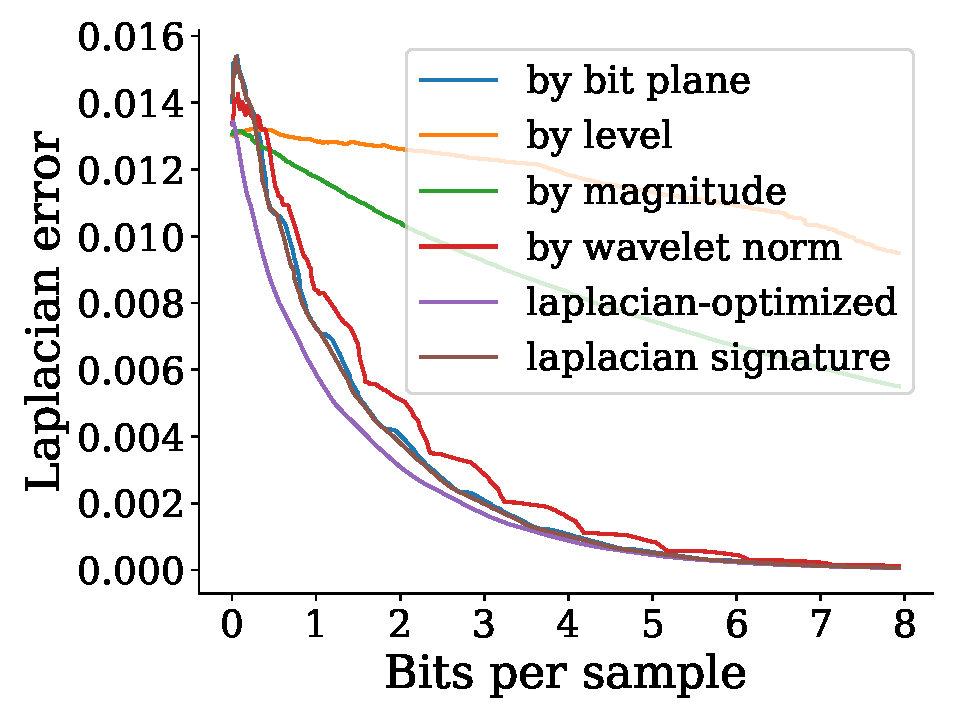
\includegraphics[width=0.48\linewidth]{laplacian/laplacian-optimized-boiler}}
	\subcaptionbox{diffusivity}
	{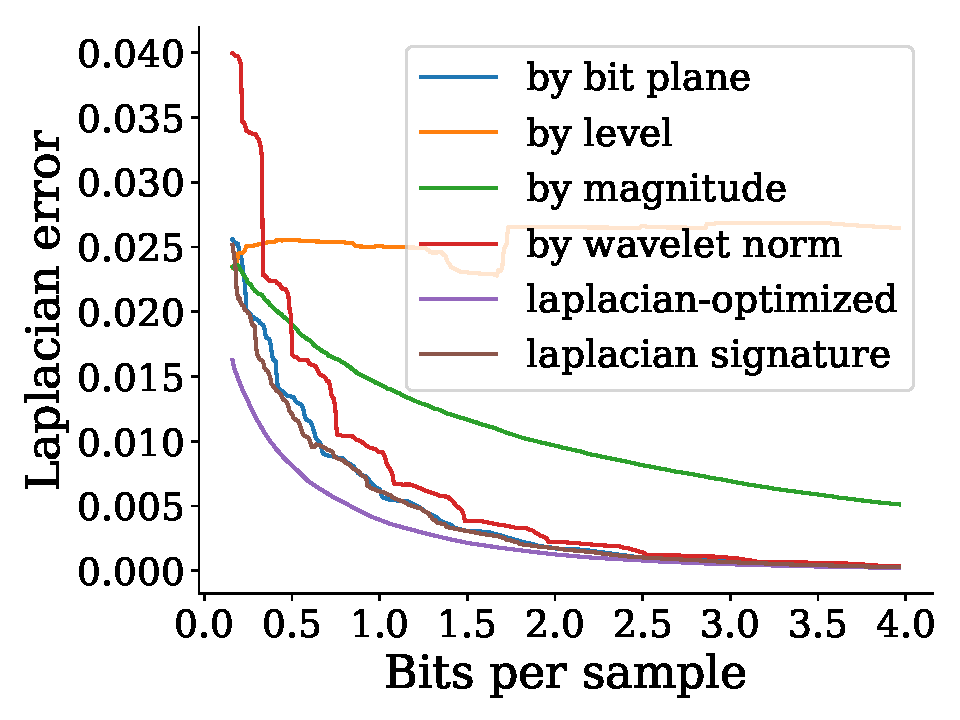
\includegraphics[width=0.48\linewidth]{laplacian/laplacian-optimized-diffusivity}}
	\subcaptionbox{turbulence}
	{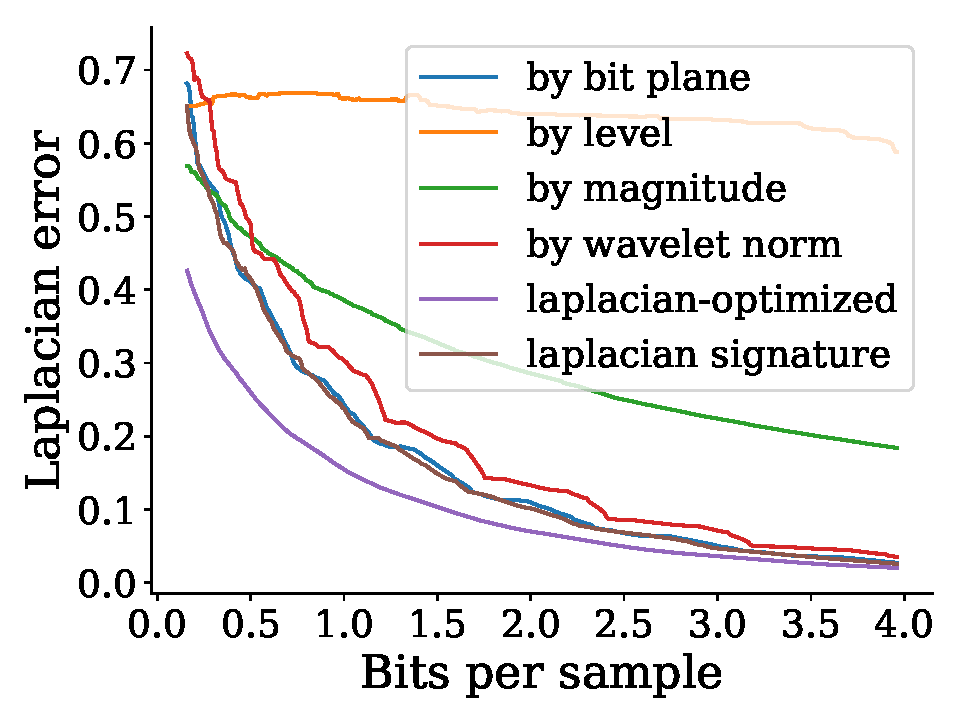
\includegraphics[width=0.48\linewidth]{laplacian/laplacian-optimized-turbulence}}
	\subcaptionbox{pressure}
	{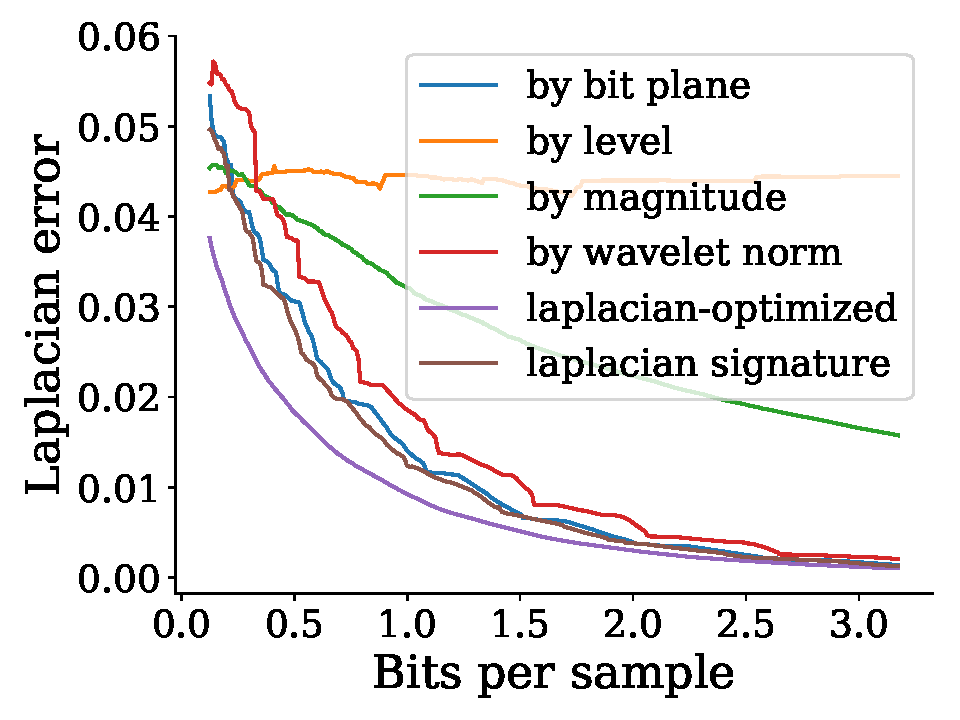
\includegraphics[width=0.48\linewidth]{laplacian/laplacian-optimized-pressure}}
	\caption{Laplacian error comparison among streams, using the three-point stencil. The plots are
	truncated so as to better highlight differences without discarding important information. In all cases, \emph{laplacian}}
	\label{fig:laplacian-error-comparison}
\end{figure}

It can be observed that unlike the case for gradient, there exists significant differences between
the \emph{rmse-optimized} and \emph{laplacian-optimized} streams with regards. To understand these
differences we plot the precision of every wavelet coefficients at a low bit rate in Figure
\ref{fig:laplacian-precision-comparison} (a and b). When cross refererencing this Figure with Figure
\ref{fig:gradient-comparison}b we see that the \emph{laplacian-optimized} stream priotizes
finer-resolution bits where the sharp shockwave is, unlike the \emph{rmse-optimized} stream which
prefers lower-ordered, coarse-resolution bits. This effect makes sense intuitively, as the
derivative operator makes functions less smooth, hence amplifing hard edges. This happens in the
gradient case too, but to a much lesser degree.

\begin{figure}[h]
	\centering
	\subcaptionbox{\emph{by level}}
	{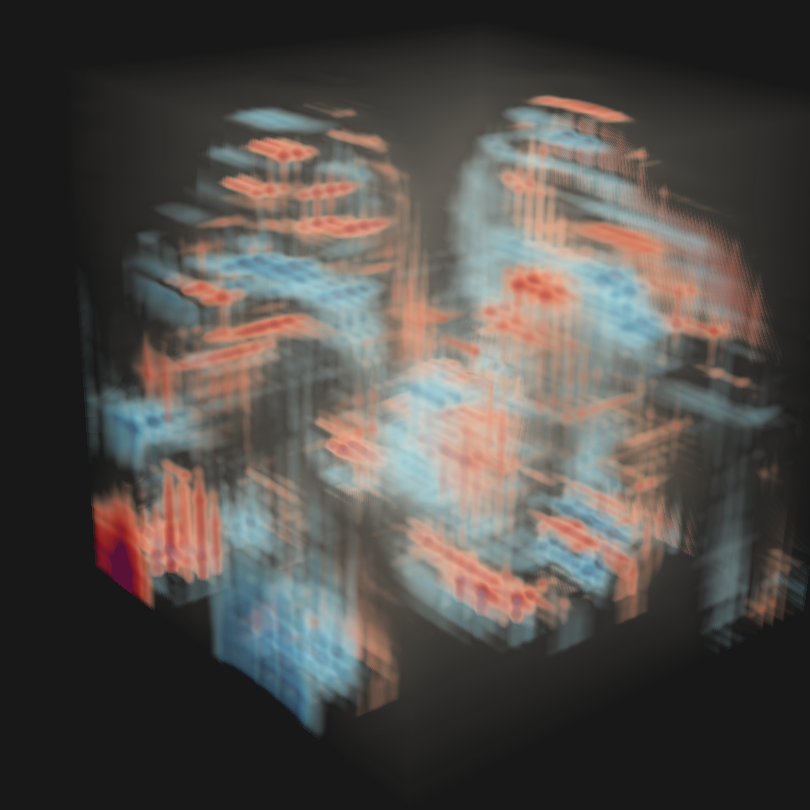
\includegraphics[width=0.31\linewidth]{laplacian/laplacian-pressure-level}}
	\subcaptionbox{\emph{by bit plane}}
	{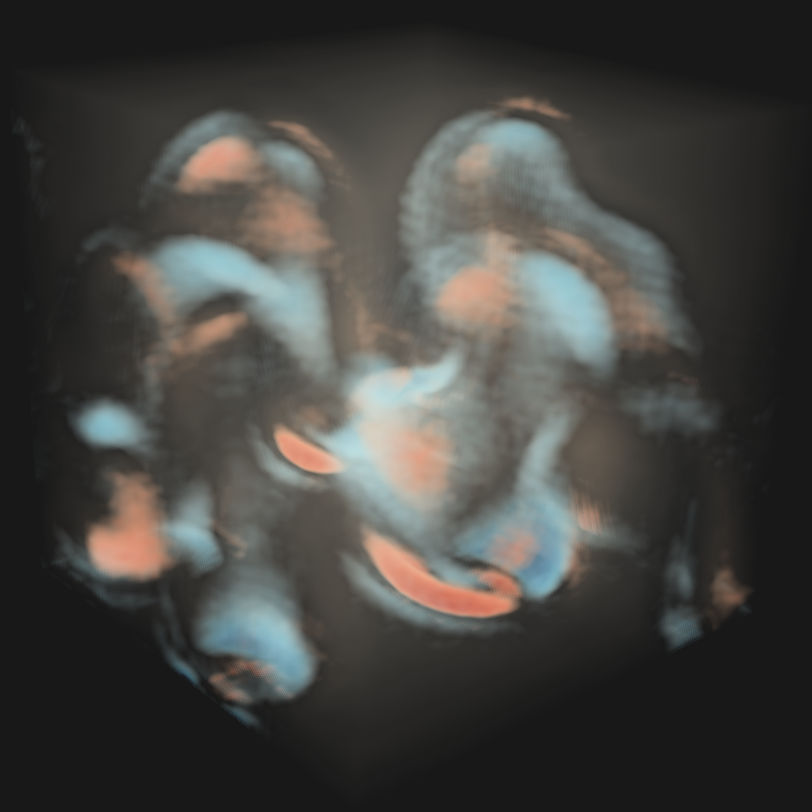
\includegraphics[width=0.31\linewidth]{laplacian/laplacian-pressure-bit-plane}}
	\subcaptionbox{\emph{by magnitude}}
	{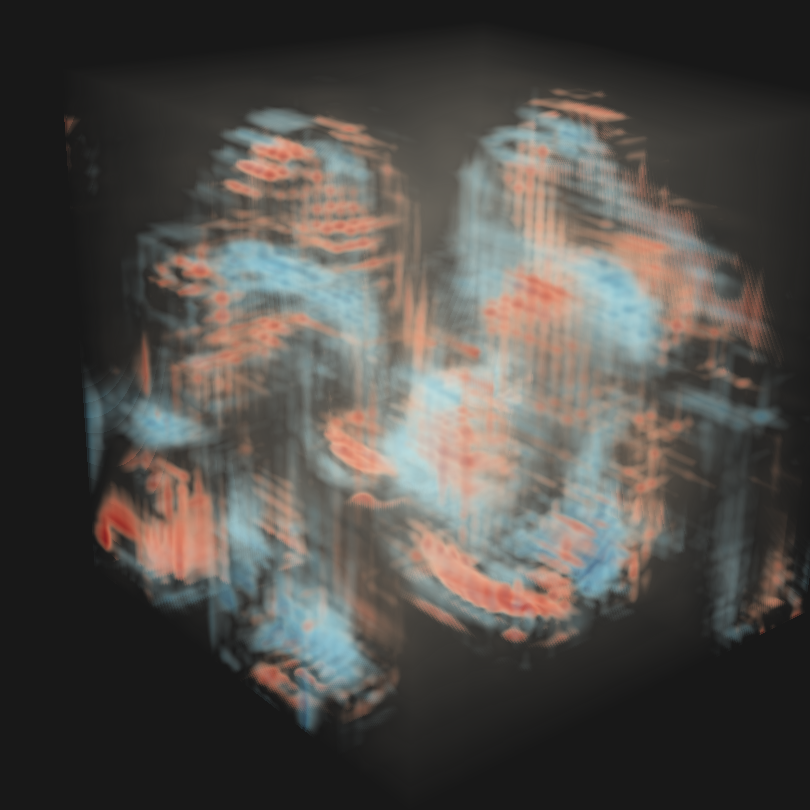
\includegraphics[width=0.31\linewidth]{laplacian/laplacian-pressure-magnitude}}
	\subcaptionbox{\emph{by wavelet norm}}
	{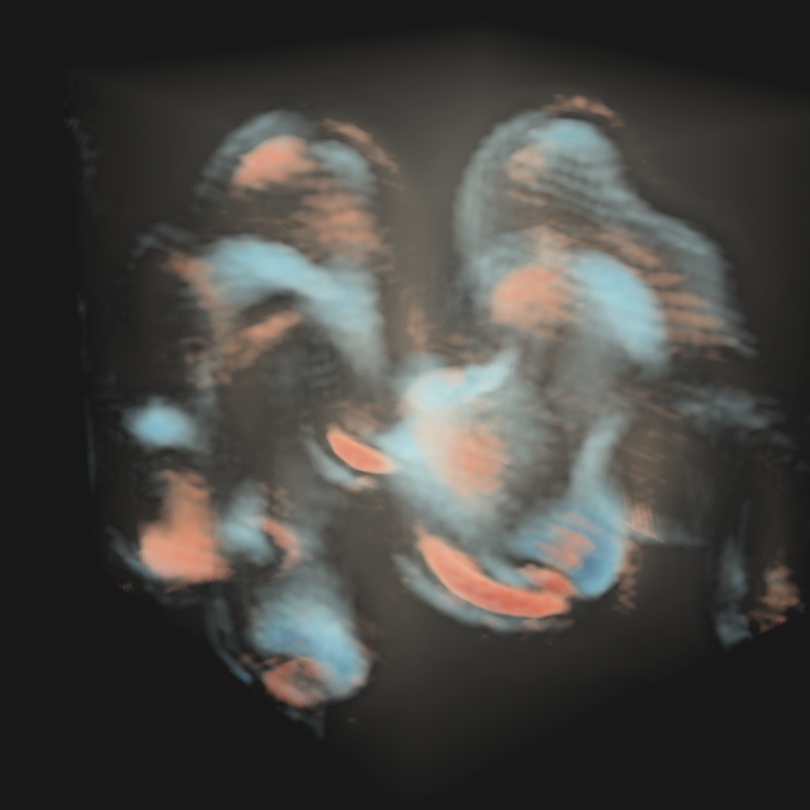
\includegraphics[width=0.31\linewidth]{laplacian/laplacian-pressure-wavelet-norm}}
	\subcaptionbox{\emph{by signature}}
	{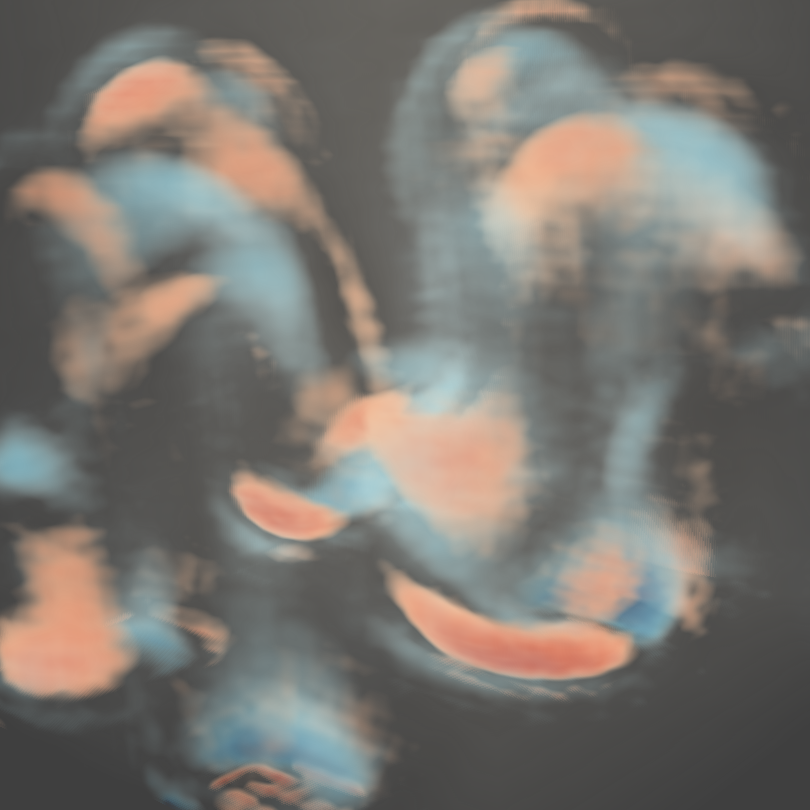
\includegraphics[width=0.31\linewidth]{laplacian/laplacian-pressure-signature}}
	\subcaptionbox{\emph{groundtruth}}
	{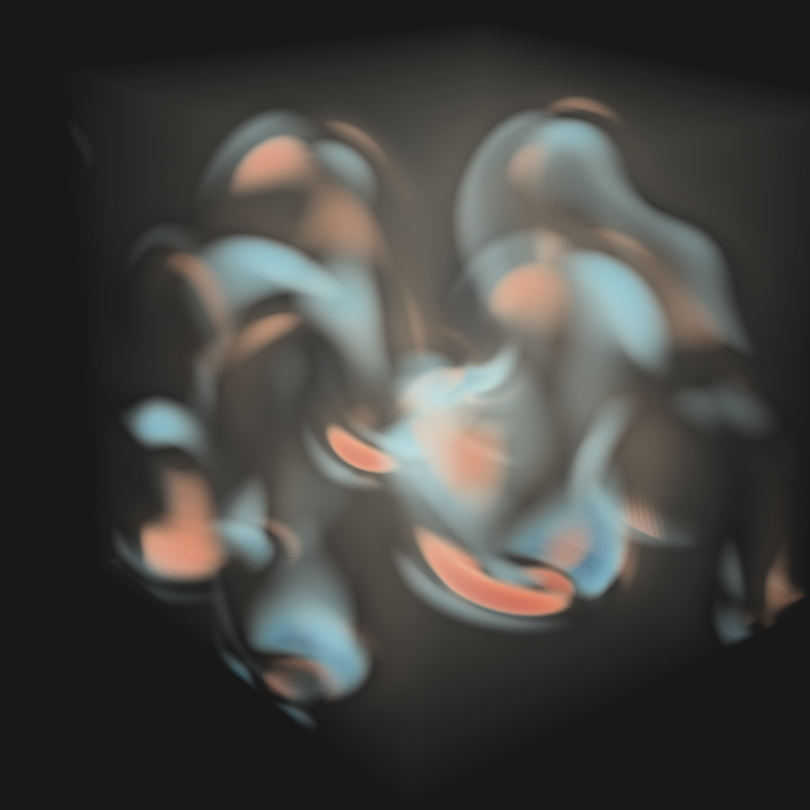
\includegraphics[width=0.31\linewidth]{laplacian/laplacian-pressure-groundtruth}}
	\caption{pressure, laplacian, 0.9 bps}
	\label{fig:laplacian-precision-comparison}
\end{figure}

\emph{rmse-optimized}, \emph{laplacian-optimized}, and also \emph{gradient-optimized} for the euler
data set are visualized in Figure \ref{fig:signature-comparison}. 

TODO: add comparison of stream signatures
% \begin{figure}[h]
% 	\centering
% 	\subcaptionbox{\emph{rmse-optimized}}
% 	{
\includegraphics[width=0.32\linewidth]{img/gradient-laplacian/SIG-GREEDY-(rmse).png}}
% 	\subcaptionbox{\emph{laplacian-optimized}}
% 	{
\includegraphics[width=0.32\linewidth]{img/gradient-laplacian/SIG-GREEDY-(laplacian).png}}
% 	\subcaptionbox{\emph{gradient-optimized}}
% 	{
\includegraphics[width=0.32\linewidth]{img/gradient-laplacian/SIG-GREEDY-(gradient).png}}
% 	\caption{Stream signatures visualized through a linear-blue color map (brighter is higher
% 	priority). From left to right: higher-ordered to lower-ordered bit planes. From top to bottom:
% 	coarser to finer subbands. Note that the streams from which the signatures are extracted do not
% 	contain leading zero bits, which explains the very dark cells }
% 	\label{fig:signature-comparison}
% \end{figure}

Using the signature for \emph{laplacian-optimized}, we are able construct a data-independent stream
(in the sense that once the signature is computed and is given, the ordering of the bits follows the
the signature only). This stream, called \emph{laplacian signature}, performs at least as well as,
and often better, than \emph{rmse-optimized} for all data sets (see Figure
\ref{fig:laplacian-comparison}). The reason \emph{laplacian signature} does not always outperform
\emph{rmse-optimized}, and that there is still a gap between itself and \emph{laplacian-optimized}
is that the signature is computed essentially by `'averaging'' local signatures, a process that
lessen the effectiveness of the signature when the data is highly inhomogenous (e.g., the euler data
set with its sharp shockwaves). Nevertheless, even with one signature for the whole domain, we are
able to reconstruct more accurate Laplacian in all cases in experiment. In practice, the signature
is a tiny piece of meta information that can be pre-computed, stored, and transmitted before any
value bits to help `'steer'' the data stream, whenever Laplacian is the quantity of interest.
